\documentclass[11pt]{article}
\usepackage{geometry}
% Math packages.
\usepackage{amsmath,amssymb,amstext,amsfonts}
% Add figures.
\usepackage{graphicx}
%needed for table stuff
\usepackage{multirow}

% Metadata
\author{Jarod Klion}
\title{Solving Matrix Equations}

\newcommand{\norm}[1]{\lVert#1\rVert}

\begin{document}

\maketitle

\section{Executive Summary}

In this report, we consider the solutions $x$ of symmetric positive definite (SPD) matrix problems, $Ax = b$, using two methods: 1.)  preconditioned steepest descent (PSD) and 2.) preconditioned conjugate gradient (PCG) with one of three preconditioners: 1.) no preconditioner, $P_I$, 2.) Jacobi's preconditioner, $P_{Jacobi}$, and 3.) symmetric Gauss-Seidel precondioner, $P_{SGS}$. Correctness of the analytic derivations is evaluated by relative error calculations depending on whether the solution is known beforehand or not. Results are obtained and discussed for 4 randomly generated SPD matrices of increasing size, and the given linear system: $A_{test} = 
\begin{bmatrix} 5 & 7 & 6 & 5 \\ 
		     7 & 10 & 8 & 7 \\
		     6 & 8 & 10 & 9 \\
		     5 & 7 & 9 & 10 \end{bmatrix}$, and
$b_{test} = \begin{bmatrix} 23 \\ 
				    32 \\
				    33 \\
				    31 \end{bmatrix}$.

\section{Statement of the Problem}

The numerical solution to the linear system $Ax = b$ is important in nearly all scientific- and mathematical-computing applications as matrices exist and are used everywhere. Preconditioned solving methods can be used to solve the linear system more computationally efficiently using no preconditioner, Jacobi's preconditioner, and the symmetric Gauss-Seidel preconditioner given by: 
\begin{itemize}
	\item $P_I = I$
	\item $P_{Jacobi}$ = diag($A$)
	\item $P_{SGS} = CC^T \Rightarrow 
		C = \begin{bmatrix} \frac{a_{11}}{\sqrt{a_{11}}} & 0 				       & \cdots & 0 \\
					 \frac{a_{21}}{\sqrt{a_{11}}} &  \frac{a_{22}}{\sqrt{a_{22}}} & \cdots & 0 \\
					 \vdots 			       & \vdots 			       & \ddots & \vdots \\
				            \frac{a_{n1}}{\sqrt{a_{11}}}&  \frac{a_{n2}}{\sqrt{a_{22}}} & \cdots & 0
		\end{bmatrix},$ 
\end{itemize} 
and the accuracy of the factorization should be the same as if the system was solved directly with inverses. We analyze the accuracy of the methods at each iteration using the relative error, which is calculated differently depending on if the solution, $x^*$, is known beforehand or not, respectively:
\begin{itemize}
	\item relative error = $\frac{\norm{x_k - x^*}_2}{\norm{x^*}_2}$
	\item relative error = $\frac{\norm{r_k}_2}{\norm{b}_2}$

\end{itemize} 

\section{Description of the Algorithms and Implementation}

The preconditioned solving methods, PSD and PCG, are translated directly into their respective functions in \textbf{Python}, which accept five arguments: (1) an SPD matrix, $A$, (2) a vector, $b$, (3) a number denoting the preconditioner type, $P$, (4) the solution vector, $x^*$, if known/desired, and (5) a float for desired accuracy level. For example, if an SPD matrix, \textbf{A}, and vector $b$ are previously defined, then \textbf{PSD(A, b, 1, None, 10e-6)} or \textbf{PCG(A, b, 1, None, 10e-6)} performs the respective method with no preconditioning and returns the numerical solution of the matrix equation as well as the relative error at each iteration until the desired accuracy, $\norm{r_k}_2 < 10^{-6}$, is reached. For the generation of the first random 10x10 and 100x100 SPD matrices, the \textbf{make\_spd\_matrix} function in scikit-learn's \emph{dataset} library was used. Additionally, another 10x10 SPD matrix was generated using a lower triangular matrix multiplied by its tranpose in order to further test the solving methods.

\section{Description of the Experimental Design and Results}

For each given matrix and solving method, the accuracies of the solution vector are calculated directly by the formulas given in section 2. This leads us to six values for each matrix as we calculate the accuracies for each of the three preconditioning methods with either of the solving methods. These results can be seen in Tables \ref{tab:k2}, \ref{tab:ktest}, \ref{tab:k10}, \ref{tab:kL}, and \ref{tab:k100}. Then, the relative error at each iteration step $k$ for each matrix type is plotted for all 3 preconditioning methods as well as the same plots but in logscale. The associated histograms of the errors are plotted in a similar fashion after. 

In Figures \ref{fig:None}, \ref{fig:Jacobi}, and \ref{fig:SGS}, the relative error for both methods, PSD and PCG, are plotted against the increasing iteration step for no preconditioner, Jacobi's preconditioner, and the SGS preconditioner, respectively. For the case of a 2x2 matrix, we see that applying a preconditioner decreases the amount of steps it takes for either method to reach the desired accuracy with the effect being much more prominent for PSD - bringing down the steps required from $\sim$13 to 1. For the case of the 4x4 given test matrix, PSD takes several hundred steps regardless of the preconditioner applied while PCG takes $\sim$4 steps regardless. For the case of solving a randomly generated 10x10 SPD matrix with PSD, Jacobi's preconditioner took the most iterations at $\sim$278 while the SGS preconditioner took the fewest at $\sim$49. Solving that same matrix with PCG instead yields much lower results with all preconditioners taking $\sim$10 iterations before reaching the desired accuracy. Lastly, for the case of solving a randomly generated 100x100 SPD matrix with PSD, using no preconditioner takes upwards of 100000 iterations while applying either preconditioner cuts that to a third or fourth of the iterations needed. Solving that same matrix with PCG instead yields drastically lower iteration values and Jacobi's preconditioner returns to taking the most steps at $\sim$100 and no preconditioner taking the fewest.

Similarly to the other figures, in Figures \ref{fig:SPD}, \ref{fig:LogSPD}, \ref{fig:HistSPD}, the relative error achieved when solving the matrix generated by the lower triangular matrix with either PSD and PCG is plotted against the iteration step. In the case of solving this type of matrix with PSD, one can see from both figure \ref{fig:SPD} and table \ref{tab:kL} that the SGS preconditioner takes far fewer iterations - an order of magnitude less - than the cases of no preconditioner or Jacobi's preconditioner. One obvious difference between the 10x10 matrices is that regardless of the preconditioner used when solving this matrix with PSD, the iteration count is much higher than it was for the 10x10 matrix generated by the scikit-learn library. However, when solving this matrix with PCG, the resulting plots look very similar to the other 10x10 matrix in terms of both relative errors at each step and the total iteration steps required.

As can be seen from the discussion above as well as some analysis of the histograms shown in Figures \ref{fig:HistNone}, \ref{fig:HistJacobi}, \ref{fig:HistSGS}, PCG takes far fewer steps to solve these matrix systems than PSD, often by an entire order of magnitude. Focusing on the idea of steepest descent, as we get closer to the actual solution values, the descent becomes less and less steep, leading to much smaller increases in accuracy per iteration which can be seen by the many occurences of near 0 error values in the histograms. As can also be expected, as the size of the matrix increasing, a larger and larger amount of steps is required to reach the desired accuracy. The outlier is the given 4x4 test matrix, where there is instantly a massive increase in accuracy for the first few steps that tapers off, taking several times more steps than the randomly generated 10x10 matrix. One explanation for this is that the given test matrix is not diagonally dominant and has a condition number, $K(A_{test})$, of about 30, leading to a 'zig-zag' between solution values and, thus, slow convergence.


Additionally, the actual solution and the numerically achieved final solutions for the test system for each method and preconditoner are shown below: \\
\underline{Actual Solution:} \\
$x^* =  	\begin{bmatrix}
		1 \\ 
		1 \\
		1 \\ 
		1
		\end{bmatrix}$ \\
\underline{No Preconditioner Results:} \\
x$_{PSD} = \begin{bmatrix}
		1.046 \\
		0.972 \\
		0.988 \\
		1.006
		\end{bmatrix}$, \quad
x$_{PCG} = \begin{bmatrix}
		1.0 \\
		1.0 \\
		1.0 \\
		1.0 
		\end{bmatrix}$ \\
\underline{Jacobi's Preconditioner Results:} \\
x$_{PSD} = \begin{bmatrix}
		1.030 \\
		0.982 \\
		0.992 \\
		1.005 
		\end{bmatrix}$ \quad
x$_{PCG} = \begin{bmatrix}
		1.0 \\
		1.0 \\
		1.0 \\
		1.0 
		\end{bmatrix}$ \\
\underline{SGS Preconditioner Results:} \\
x$_{PSD} = \begin{bmatrix}
		1.041 \\
		0.975 \\
		0.989 \\
		1.006 
		\end{bmatrix}$ \quad
x$_{PCG} = \begin{bmatrix}
		1.0 \\
		1.0 \\
		1.0 \\
		1.0 
		\end{bmatrix}$ \\


\section{Conclusions}

Our results illustrate the accuracy of the preconditioned steepest descent and preconditioned conjugate gradient method solutions to matrix systems. We found that for the case of the preconditioned steepest descent method, the SGS preconditioner gave the desired solution accuracy in the fewest iteration steps regardless of the matrix size. Similar findings were obtained for the preconditioned conjugate gradient method although the differences between preconditioners was less severe in this case. This raises the question of how to most efficiently apply the SGS preconditioner to PSD as a dense storage approach was used for the calculations as well as raising the question if SGS preconditioner is actually the best to use practically speaking when taking into account possible time-constraints. A topic not considered in this report is the timing of each method. It is possible that despite taking the fewest overall iteration steps, the calculation time per iteration step in SGS makes the preconditioner method take the longest time-wise, which would become more and more problematic as the matrix size increases. Answers to this question and related ones could be studied further in the future or, perhaps, found in the literature.

\clearpage
%%%%%%%%%%%%%%%%%%%%%%%%%%%%%%%%%%%%%%%%%%%%%%%%%%%%%%%%%%%%%%%%%%%%%%%%%%%%%%%%%%%%%%%%%%%%%%%%%%%%%%%%%%%%%%%%%%%%%%%%%%%%%%%%%%%%%%%%%%%%%%%%%%%%%%%%%%%%%%%%%%%%%%%%

\section{Tables and Figures}
\subsection{No Preconditioner Plots}

\begin{figure}[h!]
	\hspace*{-2cm}
	\centering
	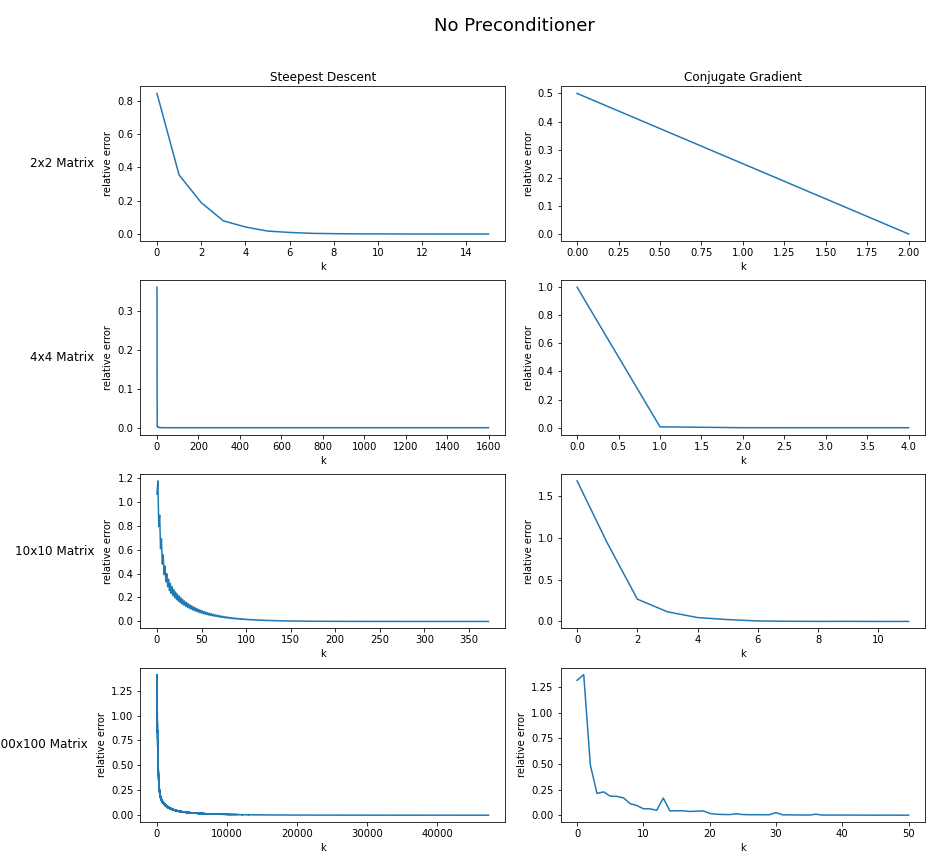
\includegraphics[width=1.1\linewidth]{../figures/No Preconditioner}
	\caption{Relative error versus the iteration number when using no preconditioner with either steepest descent (column 1) or conjugate gradient (column 2) as the solving method.}
	\label{fig:None}
\end{figure}

\begin{figure}[h!]
	\hspace*{-3cm}
	\centering
	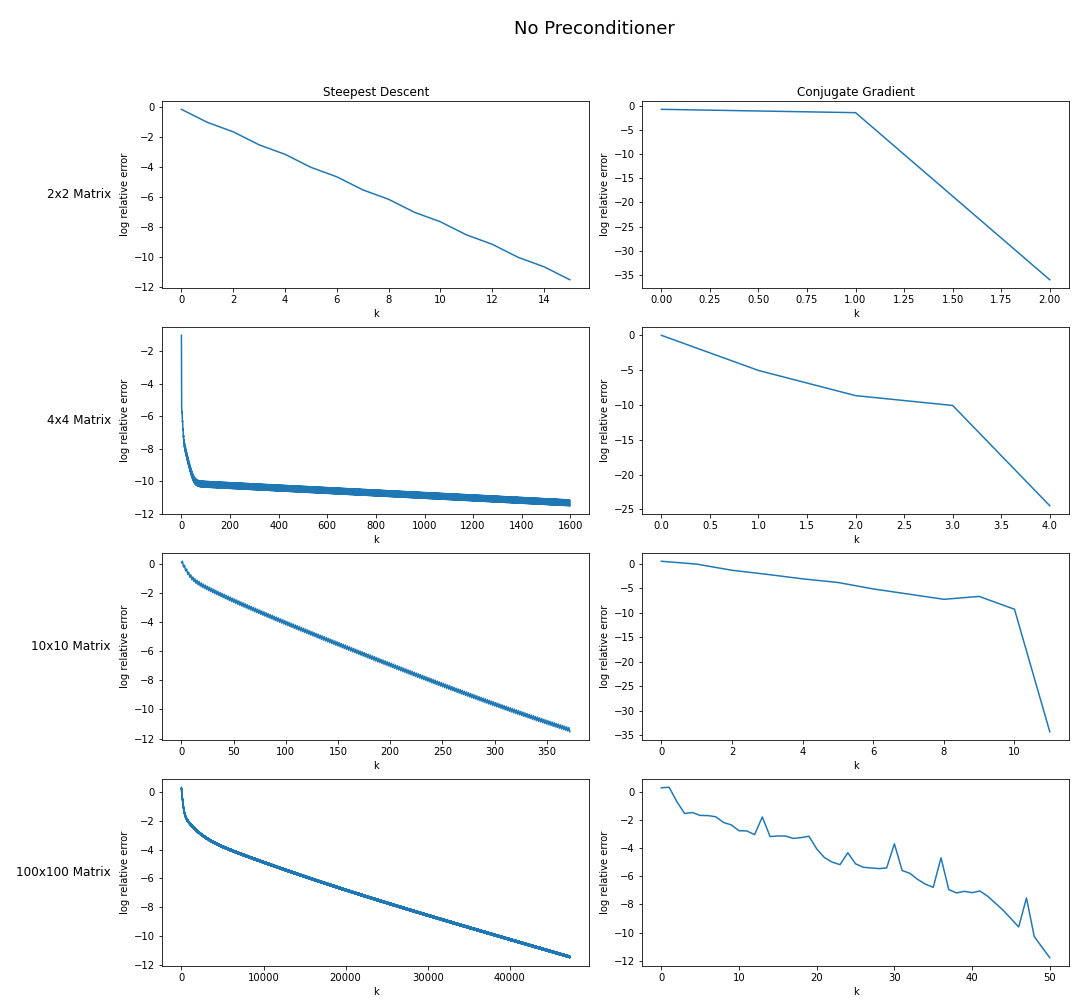
\includegraphics[width=1.3\linewidth]{../figures/Log No Preconditioner}
	\caption{Log of the relative error versus the iteration number when using no preconditioner with either steepest descent (column 1) or conjugate gradient (column 2) as the solving method.}
	\label{fig:LogNone}
\end{figure}

\begin{figure}[h!]
	\hspace*{-3cm}
	\centering
	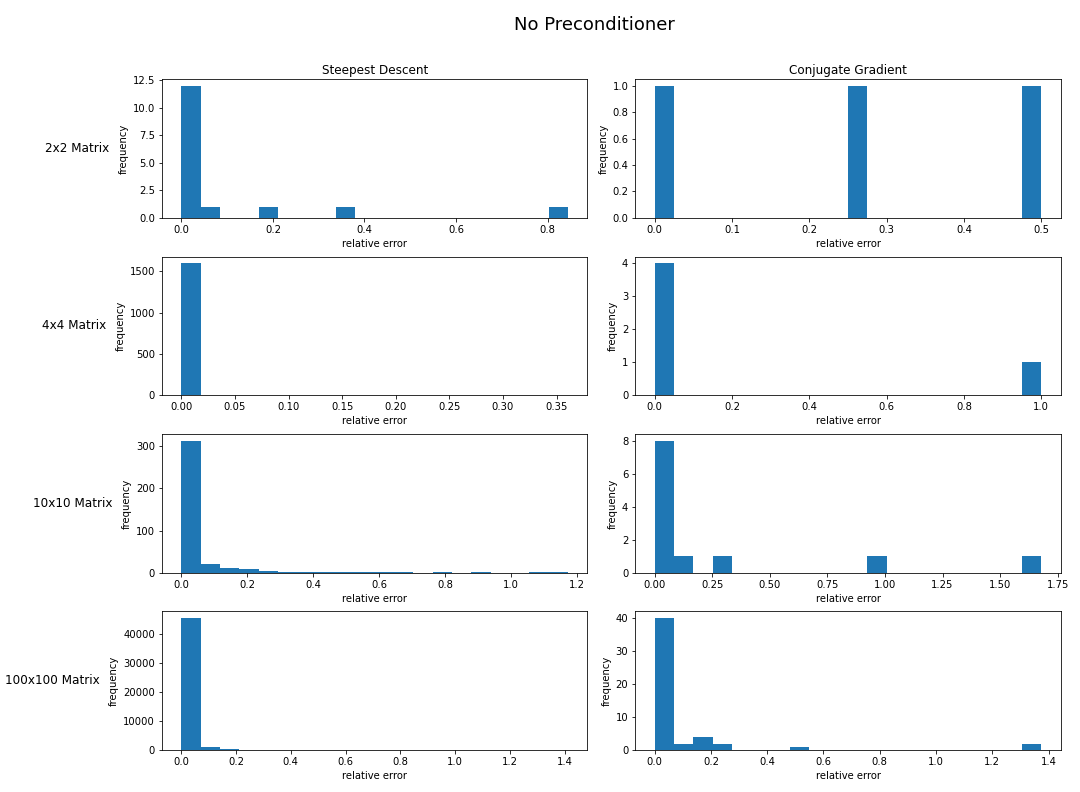
\includegraphics[width=1.3\linewidth]{../figures/No Preconditioner Histogram}
	\caption{Histogram of relative errors when using no preconditioner with either steepest descent (column 1) or conjugate gradient (column 2) as the solving method.}
	\label{fig:HistNone}
\end{figure}
\clearpage

\subsection{Jacobi's Preconditioner Plots}
\begin{figure}[h!]
	\hspace*{-2cm}
	\centering
	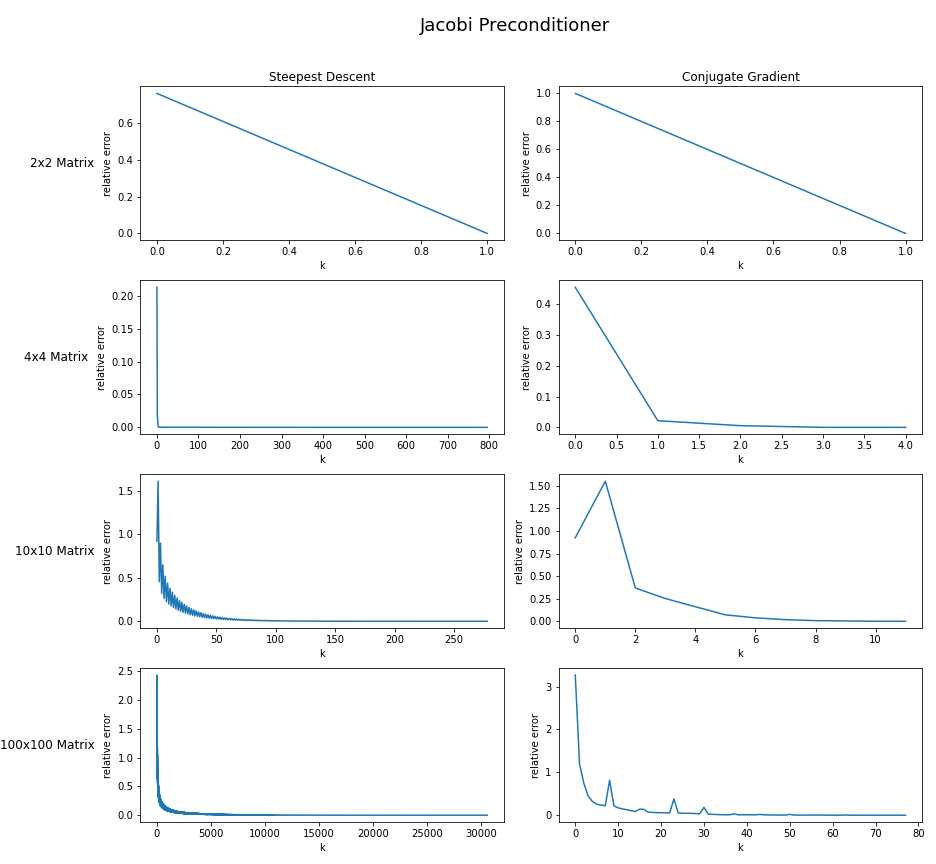
\includegraphics[width=1.2\linewidth]{../figures/Jacobi Preconditioner}
	\caption{Relative error versus the iteration number when using Jacobi's preconditioner with steepest descent (column 1) or conjugate gradient (column 2) as the solving method.}
	\label{fig:Jacobi}
\end{figure}

\begin{figure}[h!]
	\hspace*{-3cm}
	\centering
	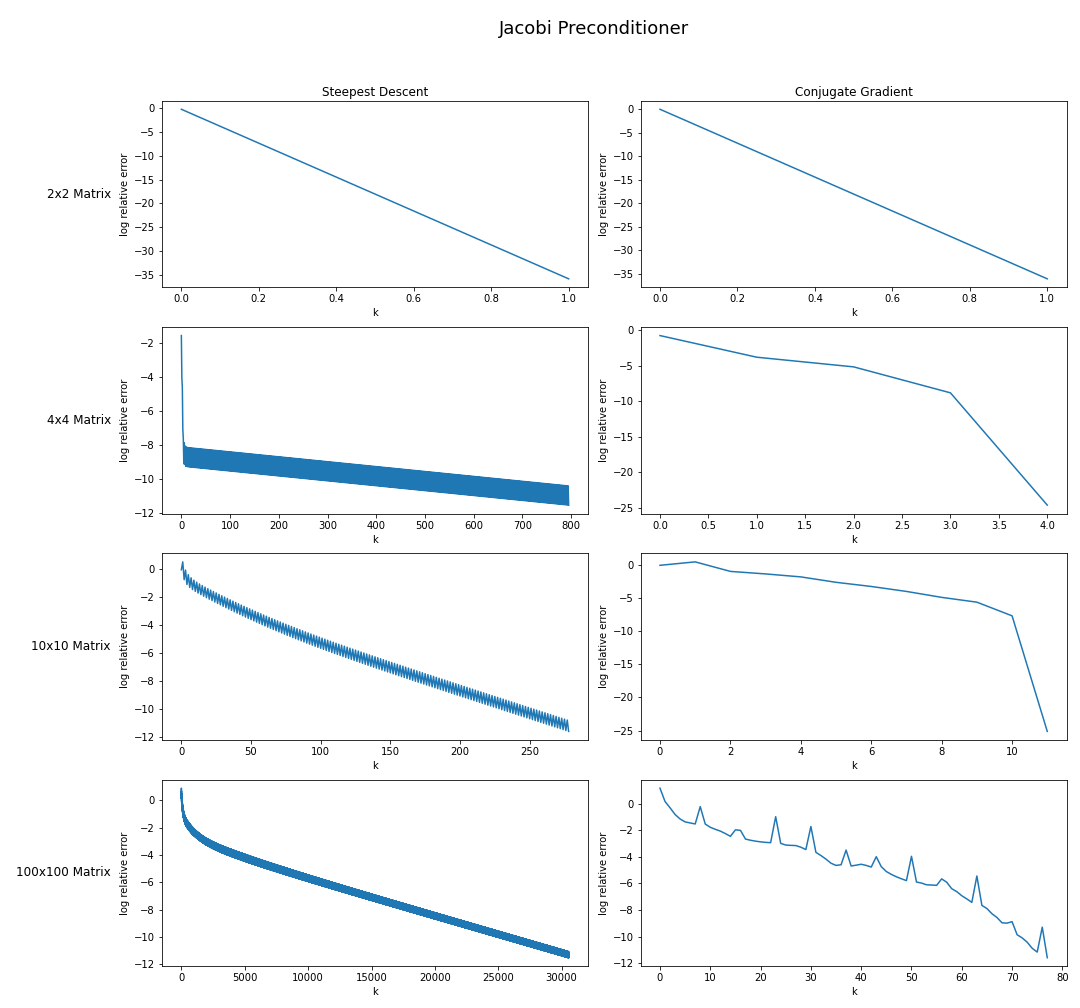
\includegraphics[width=1.3\linewidth]{../figures/Log Jacobi Preconditioner}
	\caption{Log of the relative error versus the iteration number when using Jacobi's preconditioner with steepest descent (column 1) or conjugate gradient (column 2) as the solving method.}
	\label{fig:LogJacobi}
\end{figure}

\begin{figure}[h!]
	\hspace*{-3cm}
	\centering
	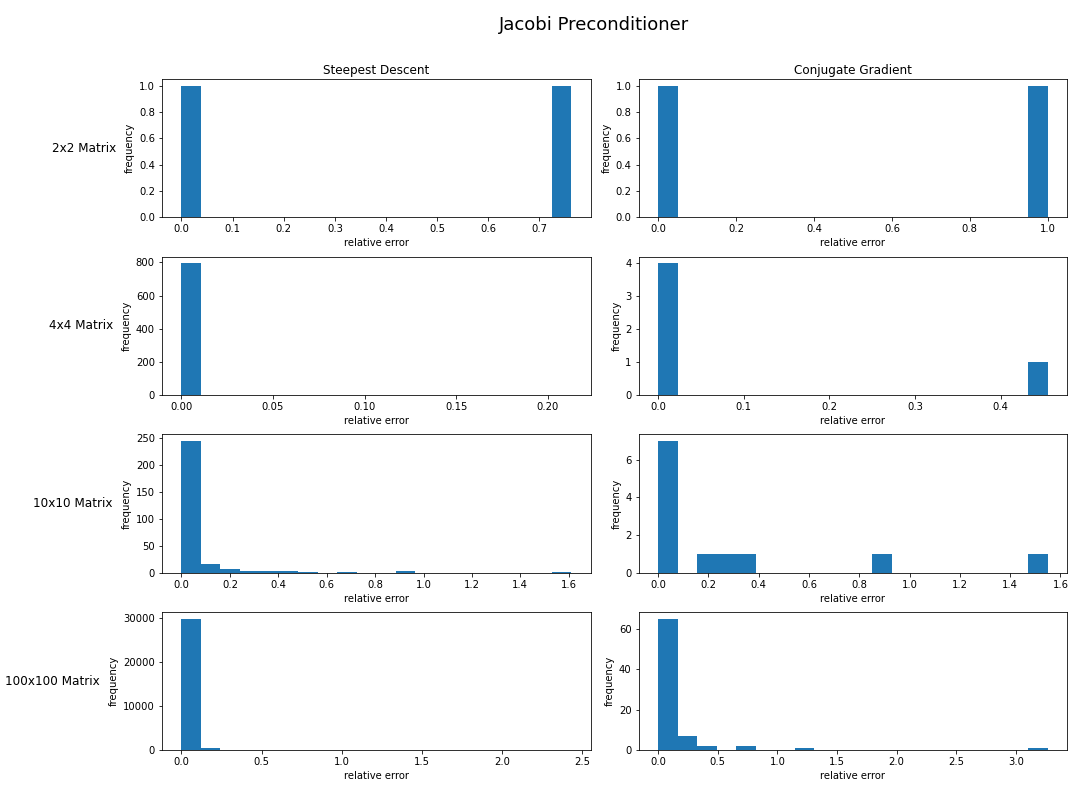
\includegraphics[width=1.3\linewidth]{../figures/Jacobi Preconditioner Histogram}
	\caption{Histogram of relative errors when using Jacobi's preconditioner with steepest descent (column 1) or conjugate gradient (column 2) as the solving method.}
	\label{fig:HistJacobi}
\end{figure}
\clearpage

\subsection{Symmetric Gauss-Seidel Preconditioner Plots}
\begin{figure}[h!]
	\hspace*{-2cm}
	\centering
	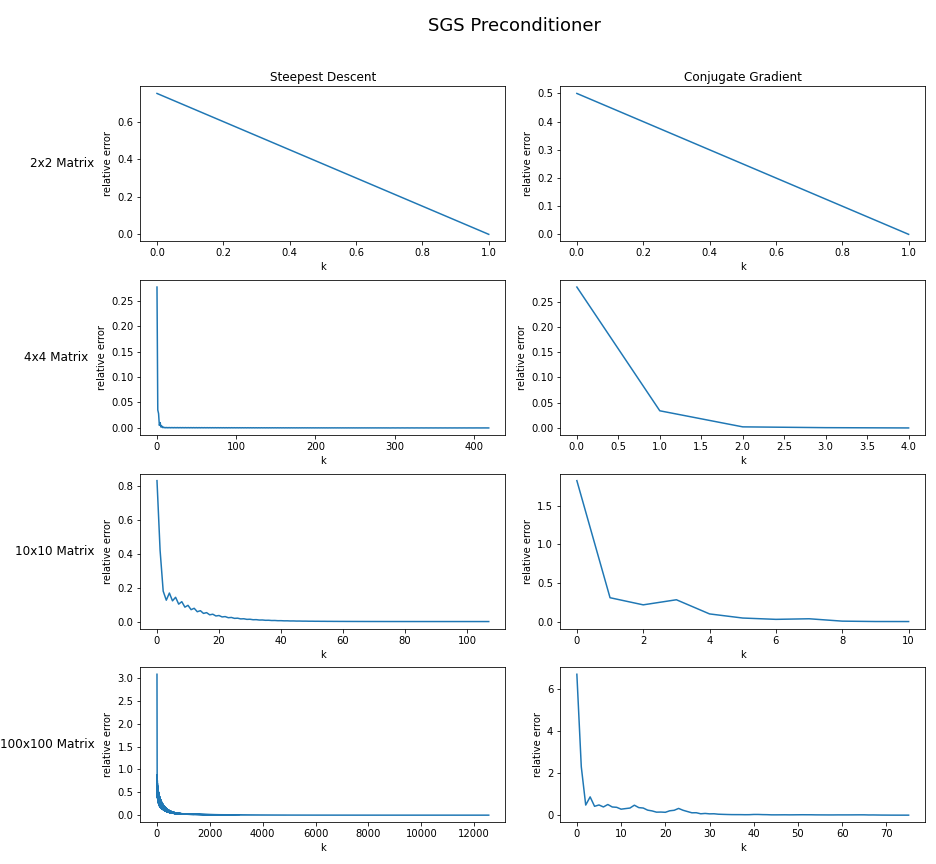
\includegraphics[width=1.2\linewidth]{../figures/SGS Preconditioner}
	\caption{Relative error versus the iteration number when using the SGS preconditioner with steepest descent (column 1) or conjugate gradient (column 2) as the solving method.}
	\label{fig:SGS}
\end{figure}

\begin{figure}[h!]
	\hspace*{-3cm}
	\centering
	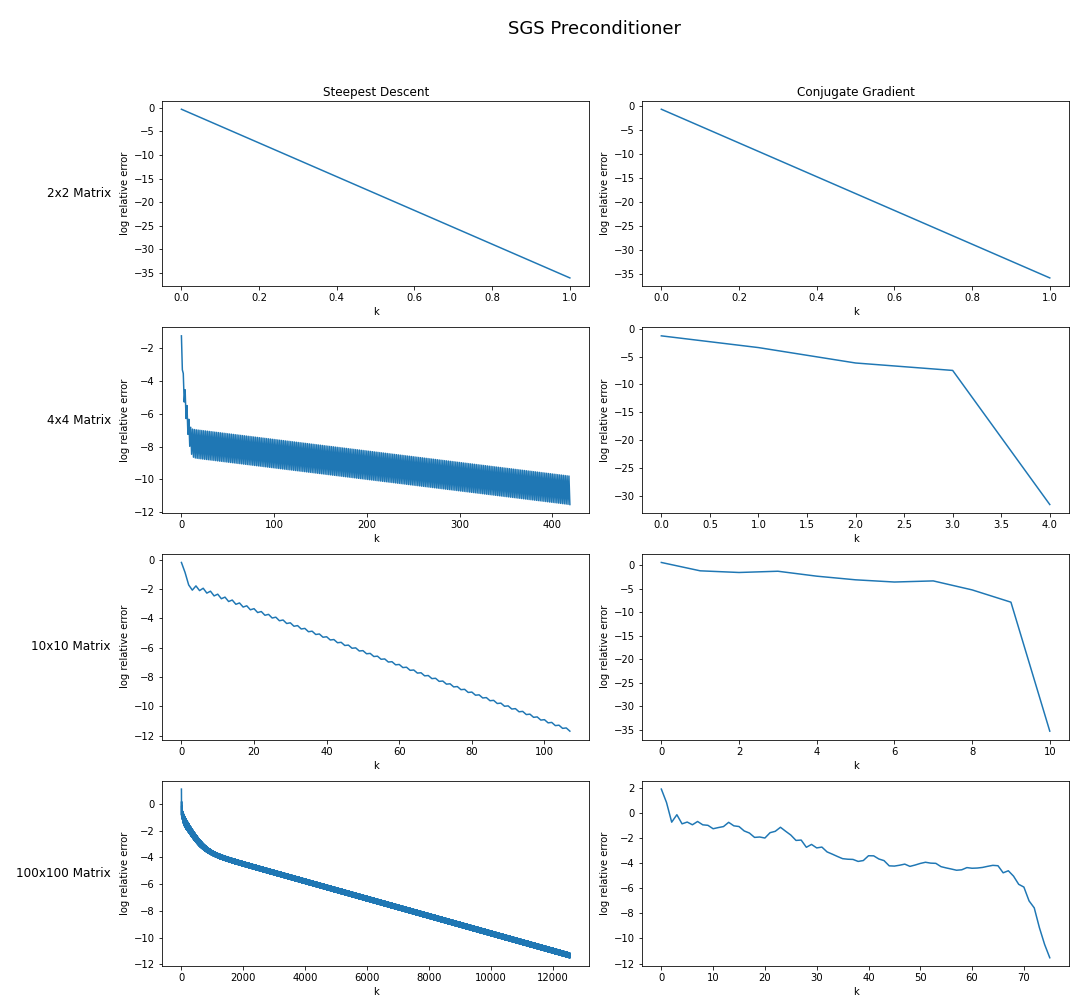
\includegraphics[width=1.3\linewidth]{../figures/Log SGS Preconditioner}
	\caption{Log of the relative error versus the iteration number when using the SGS preconditioner with steepest descent (column 1) or conjugate gradient (column 2) as the solving method.}
	\label{fig:LogSGS}
\end{figure}

\begin{figure}[h!]
	\hspace*{-3cm}
	\centering
	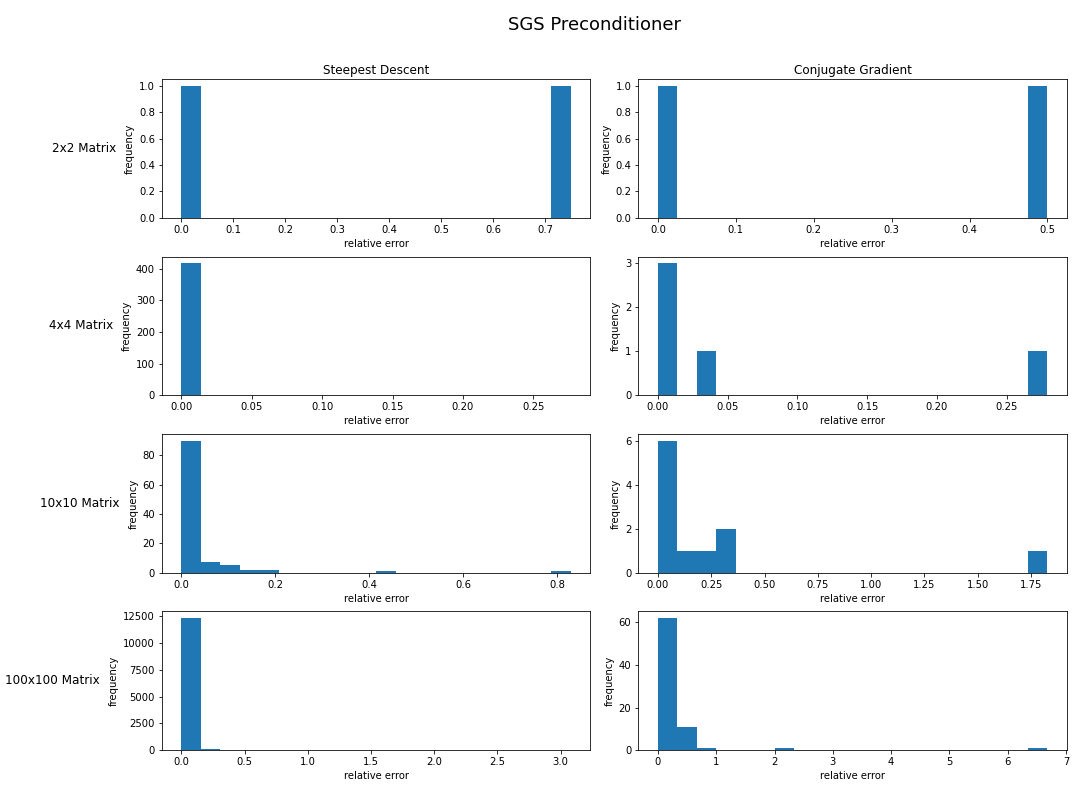
\includegraphics[width=1.3\linewidth]{../figures/SGS Preconditioner Histogram}
	\caption{Histogram of relative errors when using the SGS preconditioner with steepest descent (column 1) or conjugate gradient (column 2) as the solving method.}
	\label{fig:HistSGS}
\end{figure}
\clearpage

\subsection{SPD Matrix From $L_1$}
\begin{figure}[h!]
	\hspace*{-2cm}
	\centering
	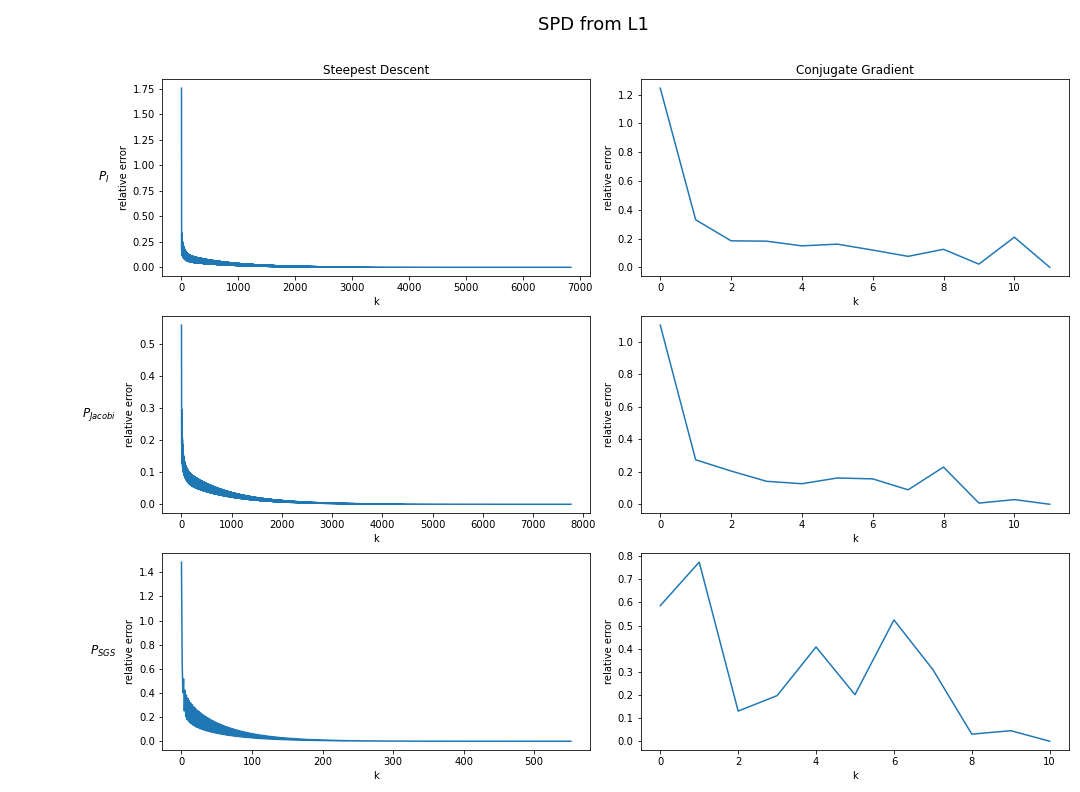
\includegraphics[width=1.2\linewidth]{../figures/SPD L1 Errors}
	\caption{Relative error versus the iteration number when using no preconditioner (row 1), Jacobi's preconditioner (row 2), or the SGS preconditioner (row 3) with steepest descent (column 1) or conjugate gradient (column 2) as the solving method.}
	\label{fig:SPD}
\end{figure}

\begin{figure}[h!]
	\hspace*{-3cm}
	\centering
	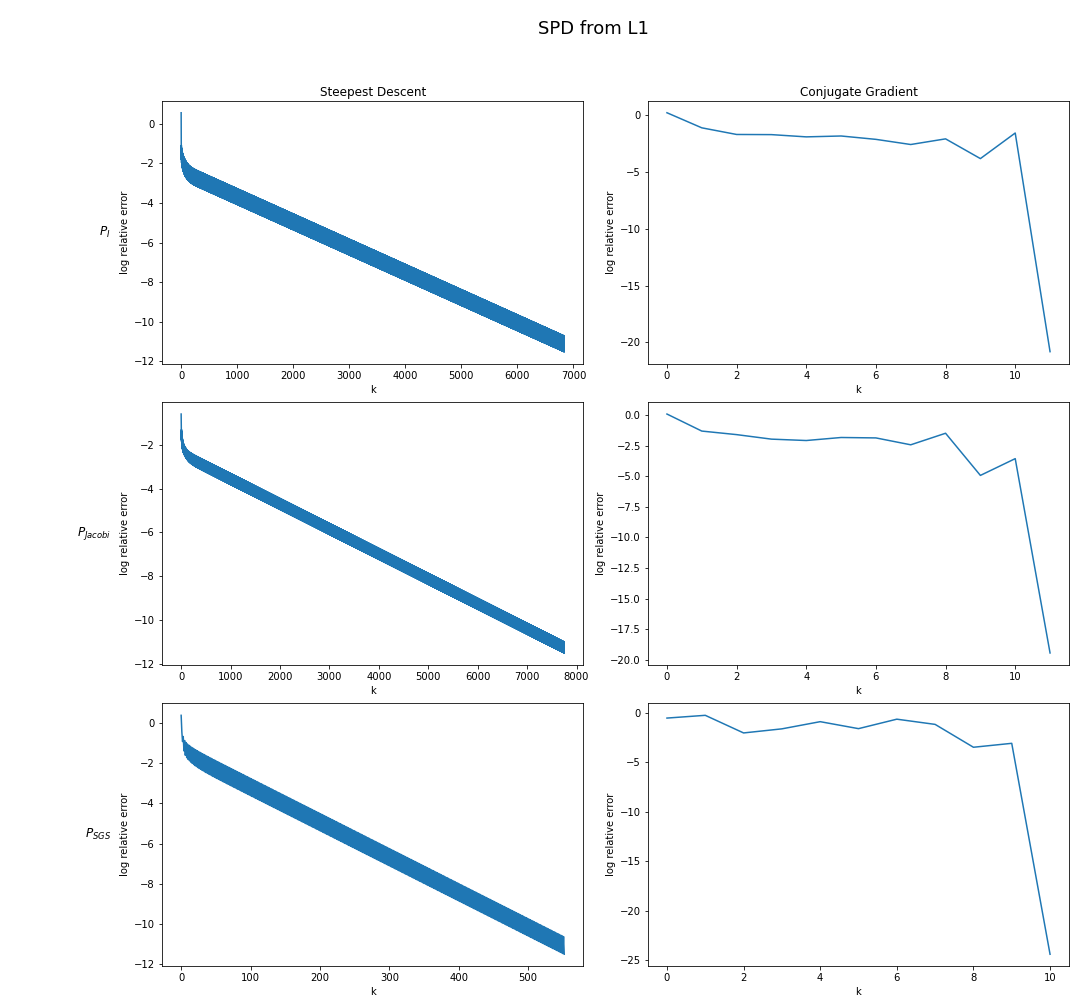
\includegraphics[width=1.3\linewidth]{../figures/Log SPD L1 Errors}
	\caption{Log of the relative error versus the iteration number when using no preconditioner (row 1), Jacobi's preconditioner (row 2), or the SGS preconditioner (row 3) with steepest descent (column 1) or conjugate gradient (column 2) as the solving method.}
	\label{fig:LogSPD}
\end{figure}

\begin{figure}[h!]
	\hspace*{-3cm}
	\centering
	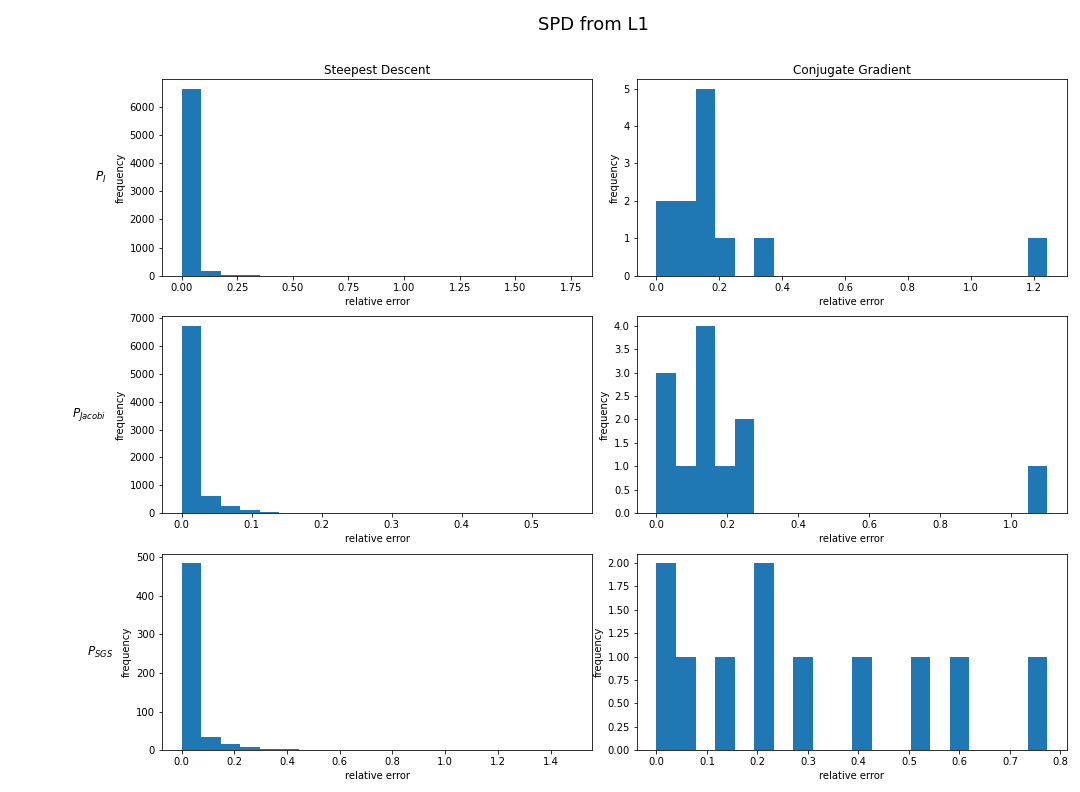
\includegraphics[width=1.3\linewidth]{../figures/SPD L1 Histogram}
	\caption{Histogram of relative errors when using no preconditioner (row 1), Jacobi's preconditioner (row 2), or the SGS preconditioner (row 3) with steepest descent (column 1) or conjugate gradient (column 2) as the solving method.}
	\label{fig:HistSPD}
\end{figure}
\clearpage



\begin{table}[h!]
	\centering
	\begin{tabular}{|c|c|c|}
	\hline
	2x2 Matrix   	 & PSD & PCG \\ \hline
	$k_I$        	 & 13  & 2   \\ \hline
	$k_{Jacobi}$ & 1   & 1   \\ \hline
	$k_{SGS}$     & 1   & 1   \\ \hline
	\end{tabular}
	\caption{Iteration counts ($k$) for each preconditioner type for preconditioned steepest descent (column 1) and preconditioned conjugate gradient (column 2) for a 2x2 matrix system.}
	\label{tab:k2}
\end{table}

\begin{table}[h!]
	\centering
	\begin{tabular}{|c|c|c|}
	\hline
	4x4 Matrix  	 & PSD  & PCG \\ \hline
	$k_I$        	 & 15085 & 11  \\ \hline
	$k_{Jacobi}$  & 16656 & 11  \\ \hline
	$k_{SGS}$     & 1363  & 10  \\ \hline
	\end{tabular}
	\caption{Iteration counts ($k$) for each preconditioner type for preconditioned steepest descent (column 1) and preconditioned conjugate gradient (column 2) for the given 4x4 matrix test system.}
	\label{tab:ktest}
\end{table}


\begin{table}[h!]
	\centering
	\begin{tabular}{|c|c|c|}
	\hline
	10x10 Matrix 	& PSD & PCG \\ \hline
	$k_I$        		& 172 & 11  \\ \hline
	$k_{Jacobi}$ 	& 278 & 10  \\ \hline
	$k_{SGS}$    	& 49  & 9   \\ \hline
	\end{tabular}
	\caption{Iteration counts ($k$) for each preconditioner type for preconditioned steepest descent (column 1) and preconditioned conjugate gradient (column 2) for a 10x10 matrix system.}
	\label{tab:k10}
\end{table}

\begin{table}[h!]
	\centering
	\begin{tabular}{|c|c|c|}
	\hline
	L1 10x10 Matrix 	& PSD  & PCG \\ \hline
	$k_I$           		& 783  & 4   \\ \hline
	$k_{Jacobi}$    	& 1192 & 4   \\ \hline
	$k_{SGS}$      	& 721  & 4   \\ \hline
	\end{tabular}
	\caption{Iteration counts ($k$) for each preconditioner type for preconditioned steepest descent (column 1) and preconditioned conjugate gradient (column 2) for a 10x10 matrix system where $A$ is generated by a lower triangular matrix such that $A = L_{1}L_{1}^T$.}
	\label{tab:kL}
\end{table}

\begin{table}[h!]
	\centering
	\begin{tabular}{|c|c|c|}
	\hline
	100x100 Matrix 	& PSD   & PCG \\ \hline
	$k_I$          		& 103742 & 65  \\ \hline
	$k_{Jacobi}$   	& 35147 & 104 \\ \hline
	$k_{SGS}$      	& 25269 & 83  \\ \hline
	\end{tabular}
	\caption{Iteration counts ($k$) for each preconditioner type for preconditioned steepest descent (column 1) and preconditioned conjugate gradient (column 2) for a 100x100 matrix system.}
	\label{tab:k100}
\end{table}



\end{document}
